%%%%%%%%%%%%%%%%%%%%%%%%%%%%%%%%%%%%%%%%%
% Beamer Presentation
% LaTeX Template
% Version 1.0 (10/11/12)
%
% This template has been downloaded from:
% http://www.LaTeXTemplates.com
%
% License:
% CC BY-NC-SA 3.0 (http://creativecommons.org/licenses/by-nc-sa/3.0/)
%
%%%%%%%%%%%%%%%%%%%%%%%%%%%%%%%%%%%%%%%%%

%----------------------------------------------------------------------------------------
%	PACKAGES AND THEMES
%----------------------------------------------------------------------------------------

\documentclass{beamer}

\mode<presentation> {
\usetheme{Madrid}
\usefonttheme{serif} 
\setbeamertemplate{navigation symbols}{} % To remove the navigation symbols from the 
}
\usepackage{lmodern}  
\usepackage{graphicx} % Allows including images
\usepackage{booktabs} % Allows the use of \toprule, \midrule and \bottomrule in tables
\usepackage[T1]{fontenc}
\usepackage[utf8]{inputenc}
\usepackage{amsmath}
\usepackage{color}
\usepackage[czech]{babel}
\usepackage{lmodern}  
\usepackage{rotating}
\usepackage{scrextend}
\usepackage{pifont}
\usepackage{hyperref}
\usepackage{bm}
\usepackage{tikz}%boxy  
\usetikzlibrary{arrows,positioning}
\usetikzlibrary{calc}
%
\newcommand*\circled[1]{\tikz[baseline=(char.base)]{
    \node[shape=circle,draw=red,inner sep=2pt] (char) {#1};}}
%
\newcommand*\circledd[1]{\tikz[baseline=(char.base)]{
    \node[shape=circle,draw=ProcessBlue, dashed, inner sep=2pt] (char) {#1};}}
%
\newcommand{\mytikzmark}[2]{%
  \tikz[remember picture,inner sep=0pt,outer sep=0pt,baseline,anchor=base] 
    \node (#1) {\ensuremath{#2}};}
%
%
\newcommand*{\boxcolor}{Red}
\makeatletter
\renewcommand{\boxed}[1]{\textcolor{\boxcolor}{%
\tikz[baseline={([yshift=-1ex]current bounding box.center)}] \node [rectangle,semithick, minimum width=1ex,draw, dashed] {\normalcolor\m@th$\displaystyle#1$};}}
 \makeatother
%
%----------------------------------------------------------------------------------------
%	TITLE PAGE
%----------------------------------------------------------------------------------------
\title[Block 6]{Praktikum z ekonometrie} % The short title appears at the bottom of every slide, the full title is only on the title page
\author{VŠE Praha} % Your name
\institute[4EK417] % Your institution as it will appear on the bottom of every slide, may be shorthand to save space
{
% Your institution for the title page
\medskip
\textit{Tomáš Formánek} % Your email address
}
\date{} % Date, can be changed to a custom date
%----------------------------------------------------------------------------------------
\begin{document}
\begin{frame}
\titlepage % Print the title page as the first slide
\end{frame}
%---------------------------------------------------------------------
\begin{frame}
\frametitle{Block 6 – Treatment effects – Outline
} % Table of contents slide, comment this block out to remove it
\tableofcontents % Throughout your presentation, if you choose to use \section{} and \subsection{} commands, these will automatically be printed on this slide as an overview of your presentation
\end{frame}

%----------------------------------------------------------------------------------------
%	PRESENTATION SLIDES
%---------------------------------------------------------------------
\section{Treatment effects: Introduction}
\begin{frame}{Treatment effects: Introduction}
\begin{itemize}
    \item Broadly speaking, treatment evaluation focuses on evaluating impact of intervention(s) on outcome(s) of interest.
    \medskip
    \item Some of the methodology and terminology comes from medical sciences.
    \medskip
    \item Typically, we are interested in measuring response to treatment, relative to some benchmark: no treatment or different treatment. 
    \medskip
    \item In economic applications, treatment and intervention are synonyms. 
    \medskip
    \item \textbf{Outcome} typically refers to (changes in) economic `status' of individuals / companies / CS units. Typically, outcome is the dependent variable in a specialized regression model.
\end{itemize}
\end{frame}
%---------------------------------------------------------------------
\begin{frame}{Treatment effects: Introduction}
\textbf{Examples of treatment} in the socio-economic context \\ \medskip
\begin{itemize}
    \item Enrollment in some form of labor training program
    \medskip
    \item Being member of trade union
    \medskip
    \item Receiving transfer payment from a social program
    \medskip
    \item Changes in regulations (imposing/alleviating restrictions)
    \medskip
    \item Being educated in small classes (as opposed to large classes) 
\end{itemize}
\bigskip
\textbf{Multiple treatments:} If treatment can vary in intensity or type. Comparing a single type of treatment to benchmark does not add complexity, yet the choice of benchmark is more flexible.
\end{frame}
%---------------------------------------------------------------------

% Define box and box title style
\tikzstyle{mybox} = [draw=blue!35, fill=white, very thick,
    rectangle, rounded corners, inner sep=1pt, inner ysep=10pt]
\tikzstyle{fancytitle} =[fill=blue!35, text=black]
%---------------------------------
\begin{frame}{Treatment effects: Types of studies}
\begin{itemize}
    \item Controlled experiments -- scientific experiments (assignment into treated and control groups is random)
    \bigskip
    \item Observational studies -- natural experiments, quasi-experiments (assignment into treatment and control group is not random) \\ \medskip
    
    Self-selection bias (treatment participation is optional, individuals who choose to participate may be systematically different from non-participant)
\end{itemize}
\end{frame}
%---------------------------------
\begin{frame}{Treatment effects: Types of studies}
\begin{tikzpicture}
\node [mybox] (box){%
\begin{minipage}{0.50\textwidth}
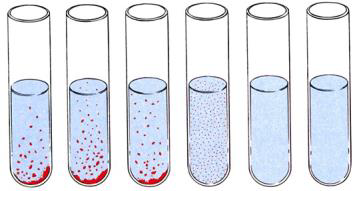
\includegraphics[width=\textwidth, height=2.89cm]{./IMG/Obrazek1}
\begin{itemize}
\scriptsize
\item Test tubes identical except for catalyst
\item Measure: Effect at different catalyst volumes (reaction speed, product volume, \dots)
\item Perform the experiment $n$-times
\item Control for other factors (heat, \dots)
\item Estimate average effect \\(\& standard error)
\end{itemize}
\end{minipage}
};
\node[fancytitle, right=5pt,  rounded corners] at (box.north west) {\scriptsize Scientific experiment};
\end{tikzpicture}%
\begin{tikzpicture}
\node [mybox] (box){%
\begin{minipage}{0.50\textwidth}
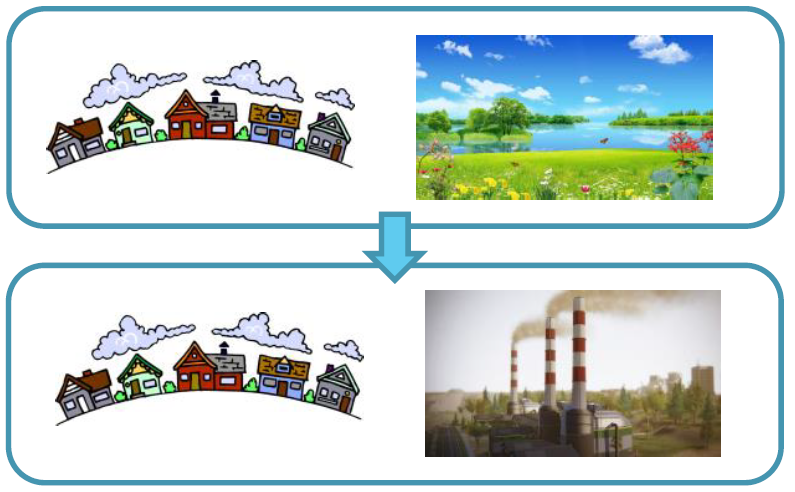
\includegraphics[width=\textwidth]{./IMG/Obrazek2}
\begin{itemize}
\scriptsize
\item Garbage incinerator is built in one given
suburban area over time
\item How do we estimate the effect on
individual house-prices?
\item Identical control group does not exist…
\item Different estimators exist\\
(assumptions apply!)
\end{itemize}
\end{minipage}
};
\node[fancytitle, right=5pt,  rounded corners] at (box.north west) {\scriptsize Natural experiment (quasi-experiment)};
\end{tikzpicture}%
\end{frame}
%---------------------------------
\section{DiD estimator: Policy analysis with pooled CS data}
\begin{frame}{DiD estimator: Policy analysis with pooled CS data}
\end{frame}
%---------------------------------
\begin{frame}{DiD estimator: Policy analysis with pooled CS data}
    describe general principle t/cont,  b/a
\end{frame}
%---------------------------------
\begin{frame}{DiD estimator: Policy analysis with pooled CS data}
\vfill
{\footnotesize \underline{\textbf{DiD estimator example: In-house employee training for women}} \\
\underline{\textbf{returning from maternal leave \& its wage effect}}} \\
\medskip
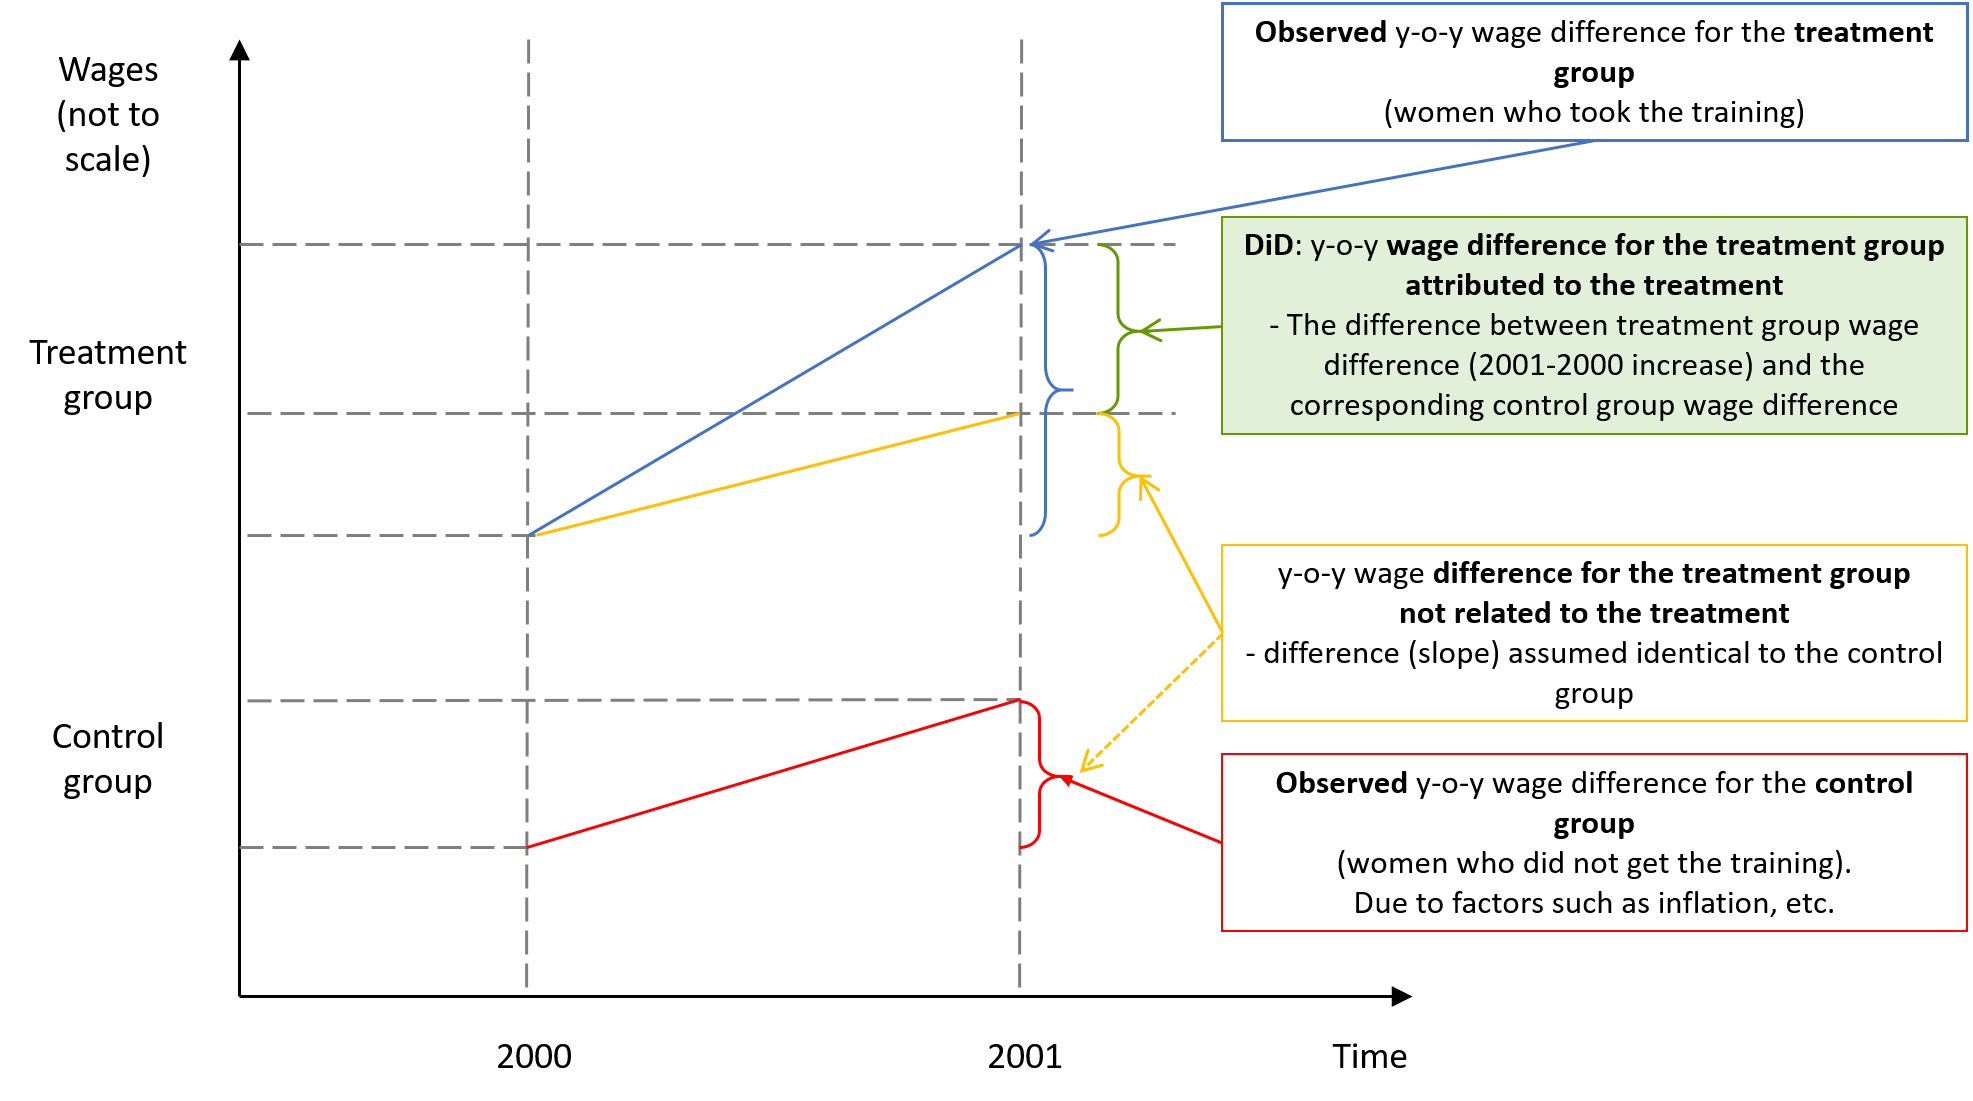
\includegraphics[width=\textwidth]{./IMG/Obrazek3}
\end{frame}
%---------------------------------
\begin{frame}{DiD estimator: Policy analysis with pooled CS data}
\underline{\textbf{DiD estimator:}} we can use LRMs to compare the changes in conditional means for the treatment and control groups…
\begin{itemize}
\item Group specific and time specific effects are allowed (controlled for)
\end{itemize}
\underline{\textbf{Assumptions:}}
\begin{itemize}
\item Unbiased DiD estimates require that the treatment (being subject to economic policy change…) is not systematically
related to factors affecting the outcome (dependent variable) that are not accounted for explicitly in our model and
thus are “hidden” in the random element.
\item DiD \textbf{attributes all differences in trends} between the treatment and control groups \textbf{to the intervention} (treatment). We assume there are no other factors that affect the difference in trends between the two groups.
\end{itemize}
\end{frame}
%---------------------------------
\begin{frame}{Example: DiD estimator}
$y_{it}=\beta_0 + \delta_0 d2 + \beta_1 dT + \delta_1 (d2 \times dT) + \bm{x}_{it} \bm{\gamma} + u_{it},$\\
\medskip
$i=1, \dots, N;~~t=1,2$. \\
\bigskip
where:
\begin{itemize}
\item[$d2$] is a dummy variable, $d2=1$ for the second period (post treatment),
\item[$dT$] is a dummy variable, equals 1 for the individuals in the treatment group,
\item[$\bm{x}_{it}$ ] is a $1 \times k$ (row) vector of additional regressors and \\
$\bm{\gamma}$ is a $k \times 1$ vector of coefficients.
\end{itemize}
\end{frame}
%---------------------------------
\begin{frame}{Example: DiD estimator}
$y_{it}=\beta_0 + \delta_0 d2 + \beta_1 dT + \delta_1 (d2 \times dT) + u_{it},$\\
\medskip
$i=1, \dots, N;~~t=1,2$. \\
\bigskip
In this simplified model (we drop $\bm{x}_{it} \bm{\gamma}$), the estimated $\delta_1$ \\has a convenient DiD interpretation:
\begin{align*}
\hat{\delta}_1 &= (\overline{y}_{Tr,\,t=2} - \overline{y}_{Co,\,t=2}) -  (\overline{y}_{Tr,\,t=1} - \overline{y}_{Co,\,t=1}), \\ ~& \\
& \hspace{0.5cm} \textnormal{which may be rearranged as:} \\ ~& \\
&= (\overline{y}_{Tr,\,t=2} - \overline{y}_{Tr,\,t=1}) -  (\overline{y}_{Co,\,t=2} - \overline{y}_{\textit{Co},\,t=1})
\end{align*}
\end{frame}
%---------------------------------
\begin{frame}{Example: DiD estimator}
$$y_{it}=\beta_0 + \delta_0 d2 + \beta_1 dT + \delta_1 (d2 \times dT) + u_{it},$$
\footnotesize
\begin{table}[]
\centering
\caption{Table: Illustration of the DiD estimator}\label{Tab1}
\begin{tabular}{|l|c|c|c|}
\hline
\multicolumn{1}{|c|}{$E(y_{it} | d2, dT)$} & Before $(t = 1)$    & After $(t=2)$                             & After - Before        \\ \hline
Control                                    & $\beta_0$           & $\beta_0 + \delta_0$                      & $\delta_0$            \\ \hline
Treatment                                  & $\beta_0 + \beta_1$ & $\beta_0 + \delta_0 + \beta_1 + \delta_1$ & $\delta_0 + \delta_1$ \\ \hline
Treatment - Control                        & $\beta_1$           & $\beta_1 + \delta_1$                      & \circled{$\delta_1$}            \\ \hline
\end{tabular}
\end{table} 

~\\
Even if $\bm{x}_{it} \bm{\gamma}$ is added back to the equation, interpretation of $\delta_1$ remains essentially unchanged.

\end{frame}
%---------------------------------
\begin{frame}{Example: DiD estimator}
\footnotesize{What is the effect of building garbage incinerator on housing prices?}
\scriptsize
\begin{table}[]
\centering
\label{Tab21}
\begin{tabular}{lclcc}
\multicolumn{3}{l}{Dependent Variable: RPRICE}                                          &                      & \multicolumn{1}{l}{}      \\
\multicolumn{3}{l}{Included observations: 321}                                          &                      & \multicolumn{1}{l}{}      \\
                                &                      & \multicolumn{1}{c}{}           &                      & \multicolumn{1}{l}{}      \\
\multicolumn{1}{c}{Variable}    & Coefficient          & \multicolumn{1}{c}{Std. Error} & t-Statistic          & \multicolumn{1}{l}{Prob.} \\
                                
                                & \multicolumn{1}{l}{} &                                & \multicolumn{1}{l}{} & \multicolumn{1}{l}{}      \\
\multicolumn{1}{c}{C}           & 82517.23             & \multicolumn{1}{c}{2726.910}   & 30.26034             & 0.0000                    \\
\multicolumn{1}{c}{Y81}         & 18790.29             & \multicolumn{1}{c}{4050.065}   & 4.639502             & 0.0000                    \\
\multicolumn{1}{c}{NEARINC}     & -18824.37            & \multicolumn{1}{c}{4875.322}   & -3.861154            & 0.0001                    \\
\multicolumn{1}{c}{Y81*NEARINC} & -11863.90            & \multicolumn{1}{c}{7456.646}   & -1.591051            & 0.1126                    \\
                                
                                & \multicolumn{1}{l}{} &                                & \multicolumn{1}{l}{} & \multicolumn{1}{l}{}      \\
R-squared                       & 0.173948             & \multicolumn{2}{l}{Mean dependent var}                & 83721.36                  \\
Adjusted R-squared              & 0.166131             & \multicolumn{2}{l}{S.D. dependent var}                & 33118.79                  \\
S.E. of regression              & 30242.90             & \multicolumn{2}{l}{Akaike info criterion}             & 23.48429                  \\
Sum squared resid               & 2.90E+11             & \multicolumn{2}{l}{Schwarz criterion}                 & 23.53129                  \\
Log likelihood                  & -3765.229            & \multicolumn{2}{l}{Hannan-Quinn criter.}              & 23.50306                  \\
F-statistic                     & 22.25107             & \multicolumn{2}{l}{Durbin-Watson stat}                & 1.557107                  \\
Prob(F-statistic)               & 0.000000             & \multicolumn{2}{l}{}                                  & \multicolumn{1}{l}{}     
\end{tabular}
\end{table}
\begin{tikzpicture}[<-,overlay,remember picture,inner sep=1.5pt,shorten <=0.2em,font=\footnotesize]
\tikzset{
    mynode/.style={rectangle,draw=blue, fill=blue!30, very thick, inner sep=.5em, minimum size=2em, text width=25em}
}
\node[mynode] at (7.8, 0.3) (Table){
\scriptsize{PRICE - house price in real terms (USD) \\ 
$Y81$ – dummy variable for $1981$, \ ($t=1978,1981$)\\
$1978$ – before ``rumors''~; $1981$ – incinerator operational \\
NEARINC – dummy for the treatment group}};
\end{tikzpicture}
\end{frame}
%---------------------------------
\begin{frame}{Example: DiD estimator}
\small
Incinerator effect on prices example, contd: \\
\medskip
The model may be easily expanded by explanatory variables such as: \textit{HOUSE.AGE, ROOMS, AREA, LOT.AREA}, etc. and the DiD interpretation remains basically unchanged \dots
\begin{block}{Selection bias (treatment effect vs. selection bias) example:}
\small
\textbf{Assumption:} “Unbiased DiD estimates require that the treatment is not systematically related to factors affecting the outcome that are not explicitly accounted for.”  \\
\medskip
Say, we have a “poor neighborhood” with relatively old and small houses and low house-prices. For complex reasons, it suffers from a representation deficit within the local city council (as compared to other “rich neighborhoods”) and is therefore more likely to get the incinerator. \\
\medskip
We do not have variables to control for this factor $\rightarrow$ the DiD estimator may be severely biased 
\end{block}
\end{frame}
%---------------------------------
\section{Regression discontinuity design}
\begin{frame}{Regression discontinuity design}
    Violates common support assumption
\end{frame}
%---------------------------------
\section{Propensity score matching}
\begin{frame}{Propensity score matching}
    
\end{frame}
%---------------------------------





%---------------------------------
\begin{frame}{Treatment effects - additional literature}
\textbf{Treatment effects}\\
\medskip
For detailed \& technical discussion, see:\\
\medskip
\begin{itemize}
\item[1.] Wooldridge: Econometric analysis of C-S and panel data, chapter 21 Estimating Average Treatment Effects
\medskip
\item[2.] Greene: Econometric analysis, chapter 19.6
\medskip
\item[3.] Angrist, Pischke: Mostly Harmless Econometrics
\medskip
\item[4.] Cameron, Trivendi: Microeconometrics, Methods and Applications, chapter 25
\end{itemize}
\end{frame}
%---------------------------------
%---------------------------------------------------------------------
\end{document}